% ============================================================
% Appendix D — TikZ Spectral Ecology Eigenfamilies
% Fun-Sphere Fantasy Engine — Preprint Figures
% Location: fun-sphere-fantasy-engine/preprints/figures/
% Author: Borealis S. Hedling
% Date: October 2026
% ============================================================

\documentclass[tikz,border=10pt]{standalone}
\usepackage{tikz}
\usetikzlibrary{matrix, positioning, arrows.meta}

\begin{document}

% ============================================================
% D.1 Spectral Ecology Manifold
% ============================================================
\begin{tikzpicture}
\node[draw, rectangle, rounded corners, align=center, text width=10cm, padding=10pt] {
$\mathcal{M}_{eco} = \{\, s \mid s \text{ is a spectral ecological state} \,\}$ \\[6pt]
Spectral ecology manifold (44D-anchored).
};
\end{tikzpicture}

\vspace{1.5cm}

% ============================================================
% D.2 Spectral Ecology Operator Table
% ============================================================
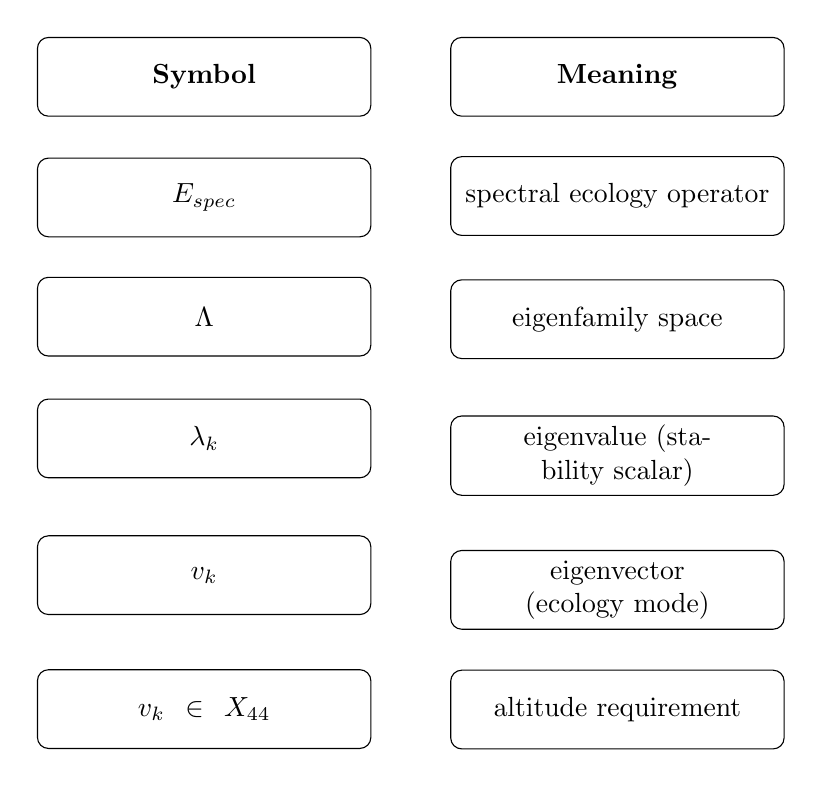
\begin{tikzpicture}
\matrix (m1) [matrix of nodes,
    nodes={draw, rectangle, rounded corners, align=center, text width=4cm, minimum height=1cm},
    column sep=1cm, row sep=0.5cm
]{
\textbf{Symbol} & \textbf{Meaning} \\
$E_{spec}$ & spectral ecology operator \\
$\Lambda$ & eigenfamily space \\
$\lambda_k$ & eigenvalue (stability scalar) \\
$v_k$ & eigenvector (ecology mode) \\
$v_k \in X_{44}$ & altitude requirement \\
};
\end{tikzpicture}

\vspace{1.5cm}

% ============================================================
% D.3 Eigenfamily Definition Block
% ============================================================
\begin{tikzpicture}
\node[draw, rectangle, rounded corners, align=center, text width=12cm, padding=10pt] {
Eigenfamily definition:\\[6pt]
$E_{spec}(v_k) = \lambda_k v_k$ \\[6pt]
High $\lambda_k$ = stable ecology; low $\lambda_k$ = unstable; negative $\lambda_k$ = catastrophic.
};
\end{tikzpicture}

\vspace{1.5cm}

% ============================================================
% D.4 Ecology-Resonance Lift Pipeline
% ============================================================
\begin{tikzpicture}[
    node distance=2.5cm,
    every node/.style={draw, rectangle, rounded corners, padding=6pt, align=center}
]

\node (r) {$r_\alpha$\\NDH resonance field\\(42D)};
\node (lu) [right=of r] {$L_u(r_\alpha)$\\semantic lift\\(43D)};
\node (c) [right=of lu] {$C(L_u(r_\alpha))$\\coherence binding\\(44D)};
\node (vk) [right=of c] {$v_k$\\spectral ecology mode};

\draw[-{Latex}] (r) -- node[above] {$L_u$} (lu);
\draw[-{Latex}] (lu) -- node[above] {$C$} (c);
\draw[-{Latex}] (c) -- node[above] {$v_k$} (vk);

\end{tikzpicture}

\vspace{1.5cm}

% ============================================================
% D.5 Monster Ecology Modes Table
% ============================================================
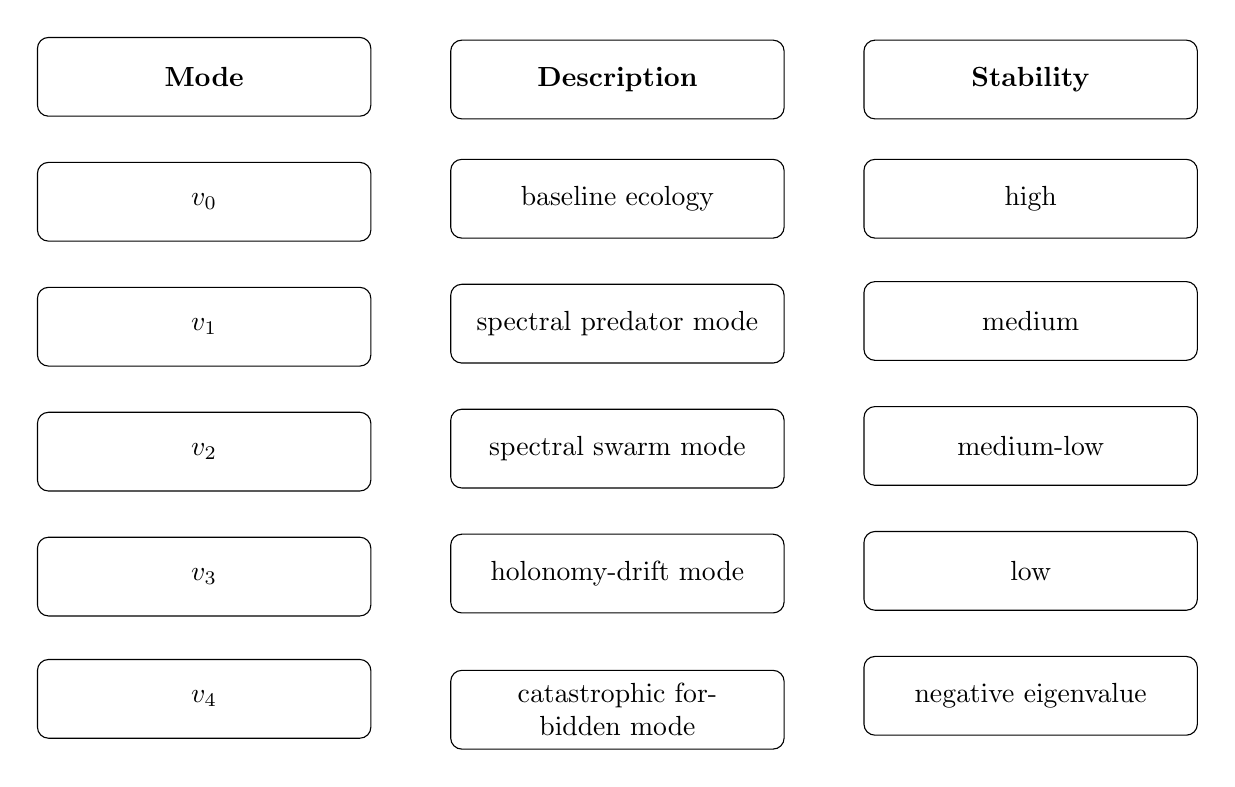
\begin{tikzpicture}
\matrix (m2) [matrix of nodes,
    nodes={draw, rectangle, rounded corners, align=center, text width=4cm, minimum height=1cm},
    column sep=1cm, row sep=0.5cm
]{
\textbf{Mode} & \textbf{Description} & \textbf{Stability} \\
$v_0$ & baseline ecology & high \\
$v_1$ & spectral predator mode & medium \\
$v_2$ & spectral swarm mode & medium-low \\
$v_3$ & holonomy-drift mode & low \\
$v_4$ & catastrophic forbidden mode & negative eigenvalue \\
};
\end{tikzpicture}

\vspace{1.5cm}

% ============================================================
% D.6 Collapse Behavior Under Ternary Projection
% ============================================================
\begin{tikzpicture}
\node[draw, rectangle, rounded corners, align=center, text width=12cm, padding=10pt] {
Ternary projection collapse:\\[6pt]
$\Pi(v_k) = \Pi(C(L_u(r_\alpha))) = \Pi(r_\alpha)$ \\[6pt]
Altitude, coherence, eigenfamilies, and ecology stability are destroyed.
};
\end{tikzpicture}

\vspace{1.5cm}

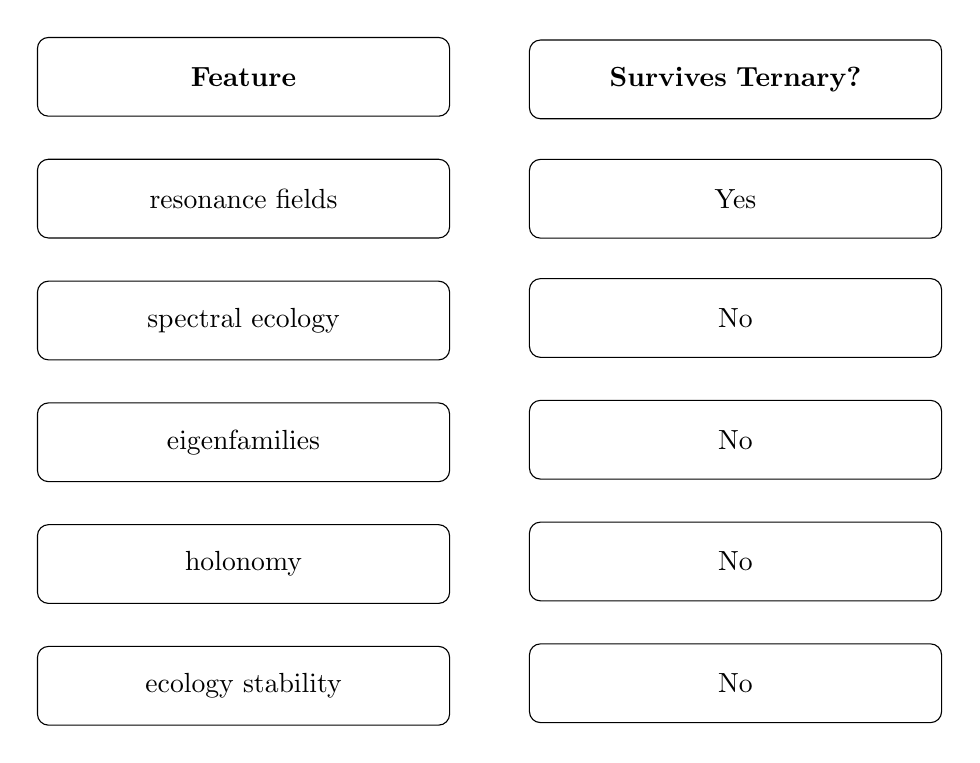
\begin{tikzpicture}
\matrix (m3) [matrix of nodes,
    nodes={draw, rectangle, rounded corners, align=center, text width=5cm, minimum height=1cm},
    column sep=1cm, row sep=0.5cm
]{
\textbf{Feature} & \textbf{Survives Ternary?} \\
resonance fields & Yes \\
spectral ecology & No \\
eigenfamilies & No \\
holonomy & No \\
ecology stability & No \\
};
\end{tikzpicture}

\vspace{1.5cm}

% ============================================================
% D.7 Stability Conditions Block
% ============================================================
\begin{tikzpicture}
\node[draw, rectangle, rounded corners, align=center, text width=12cm, padding=10pt] {
Spectral ecology stability requires:\\[6pt]
$\lambda_k > 0$ \\[4pt]
$v_k \in X_{44}$ \\[4pt]
$G(v_k) \in X_{45}$ \\[6pt]
42D cannot satisfy stability conditions.
};
\end{tikzpicture}

\vspace{1.5cm}

% ============================================================
% D.8 Summary Block
% ============================================================
\begin{tikzpicture}
\node[draw, rectangle, rounded corners, align=center, text width=13cm, padding=12pt] {
Appendix D establishes spectral ecology as a 44D phenomenon.\\[6pt]
Eigenfamilies encode monster ecology physics.\\
Ternary projection collapses all spectral ecology.\\
Fun-Sphere stability requires positive eigenvalues and altitude lift.\\
NDH resonance fields must be lifted and cohered before ecology emerges.
};
\end{tikzpicture}

\end{document}
